\documentclass{standalone}
\usepackage{tikz}
\begin{document}
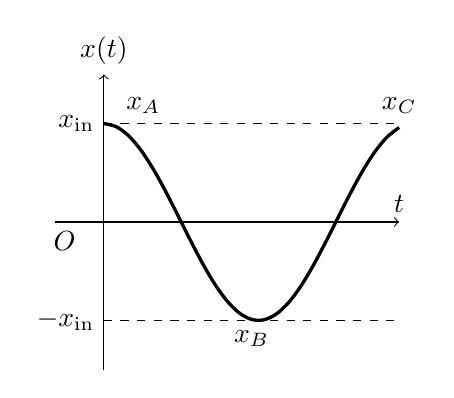
\begin{tikzpicture}[scale=2.5]
    \node[below] at (-3.2,0) {$O$};
    \draw[->] (-3.25, 0) -- (-1.5, 0) node[above]{$t$};
    \draw[->] (-3,-0.75)--(-3,0.75)node[above]{$x(t)$};

    \node[above]at(-2.8,0.5){$x_A$};
    \node[below]at(-2.25,-0.5){$x_B$};

    \draw[very thick] plot[smooth, domain=-3:-1.5] (\x, {0.5*cos(4*(\x+3) r)});

    \draw[dashed] (-3,0.5) node[left] {$x_\mathrm{in}$} -- (-1.5,0.5) node[above]{$x_C$};
    \draw[dashed] (-3,-0.5) node[left] {$-x_\mathrm{in}$} -- (-1.5,-0.5);
\end{tikzpicture}
\end{document}